\section{Introduction}
\label{sec:intro}

This paper addresses the problem of automatically building $3$D mesh models of plant leafs using inexpensive time-of-flight RGB-D sensors.  Plant researchers, seeking to understand genetic underpinnings of plant growth [REF] and seeking to develop new varieties [REF], need automated ways to non-invasively measure plant phenotypes including growth, leaf distributions, orientations, photosynthesis and productivity [REF].  An important step in estimating all of these properties is obtaining $3$D shape and pose for all the plant leafs.  Plants cannot be moved or disturbed in growth chambers, and so our concept is to mount close-range RGB-D sensors in the chambers and acquire 3D mesh models of the leafs.

Time-of-flight RGB-D sensors have both advantages and drawbacks compared to other 3D sensors.  [Expand the below]
\begin{itemize}
\item Dense depth image without scanning or rotating the target
\item Depth even on non-textured regions
\item Closely-aligned high resolution color image
\item Near IR reflectance image
\item Significantly higher depth error than laser scanners
\item Short range and sensitive to specular artifacts
\item Occlusion boundary artifacts (as with most ranging devices)
\end{itemize}

Here we address a key obstacle in obtaining accurate leaf models: the large noise in the depth images. [Expand the below:]
\begin{itemize}
\item There has been research in merging depth maps from multiple views and in reducing noise this way.  This is not so helpful here as the sensor is fixed, and the size of the noise compared to the features we want to observe is large in our application.
\item More ...
\end{itemize}

Our solution is a new mesh generation algorithm that leverages the high resolution color image, the dense depth estimates and the near-IR reflection image to overcome large depth errors.  The paper is organized as follows. [Explain]


\begin{figure}
\begin{center}
\begin{tabular}{ c c }
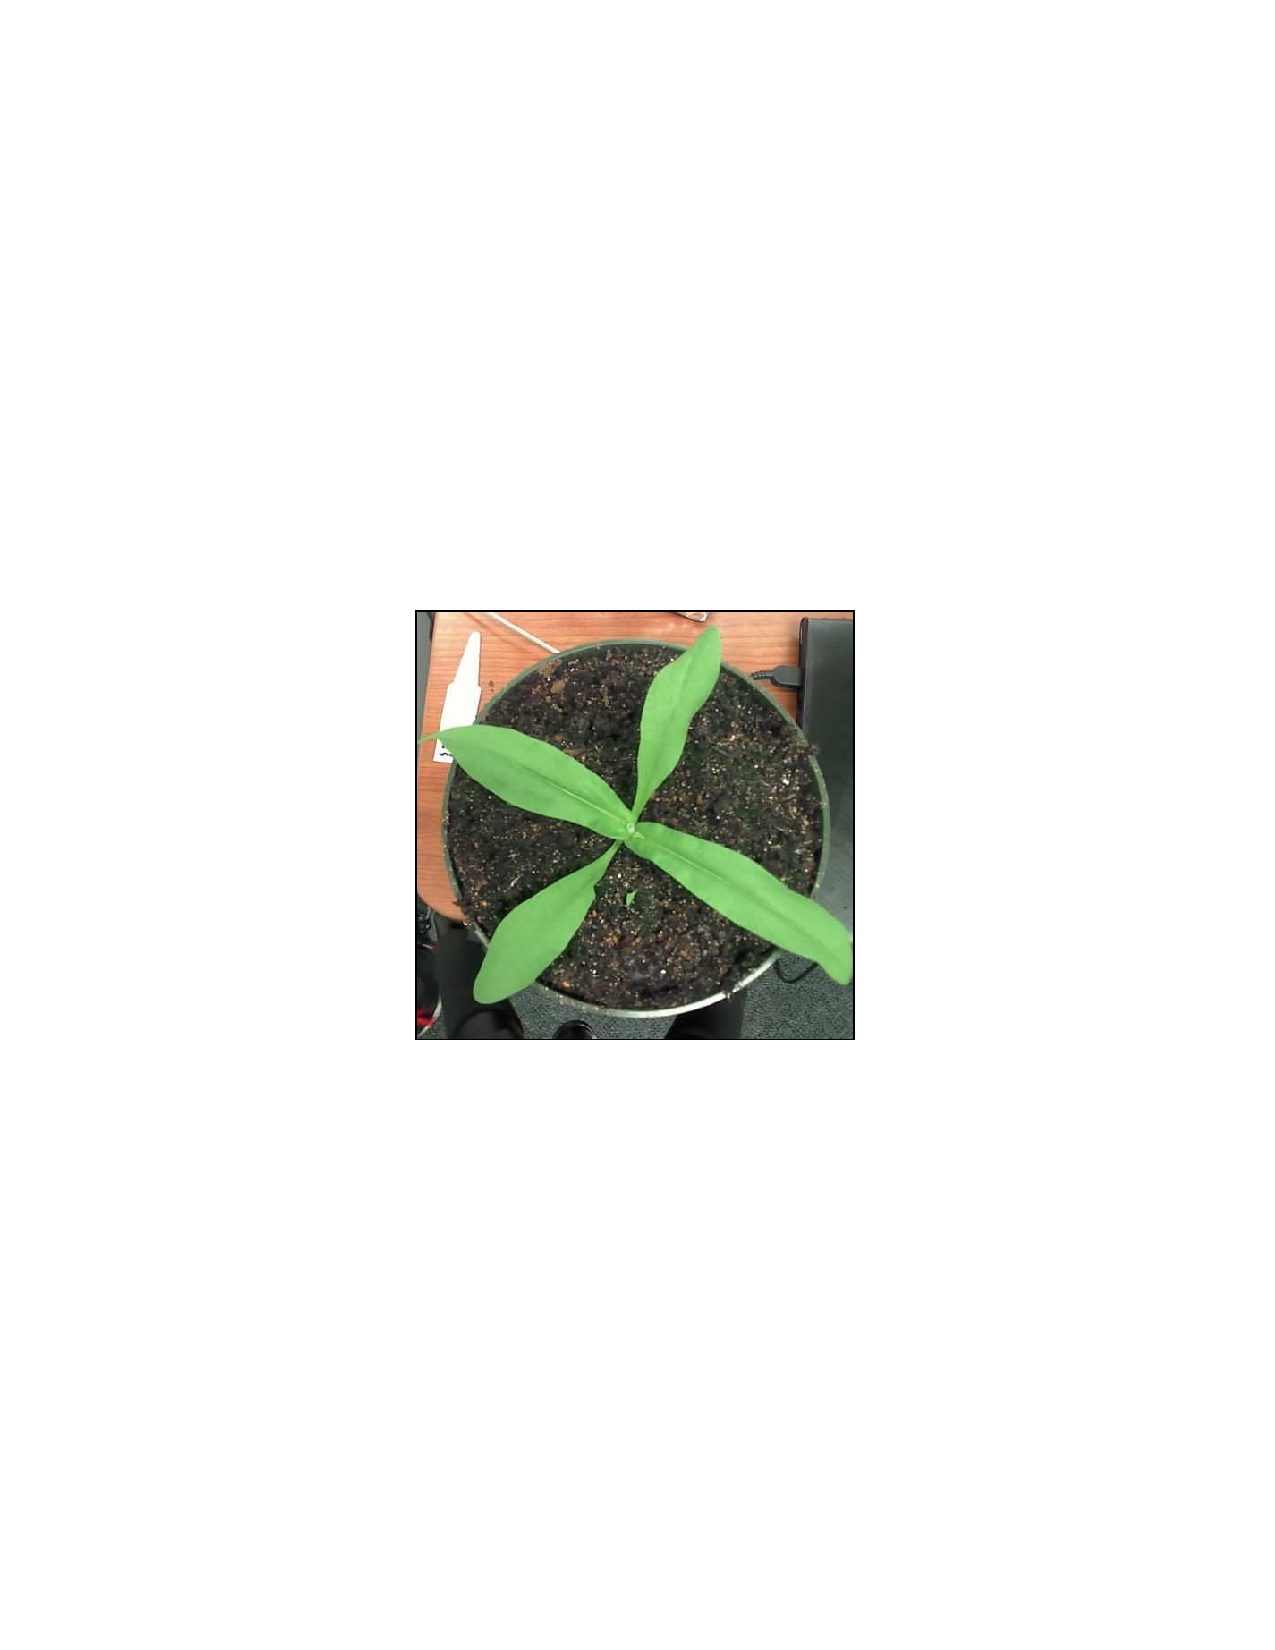
\includegraphics[trim=200 280 200 280,clip,width=0.4\linewidth]{Figures/plant1-rgb} &
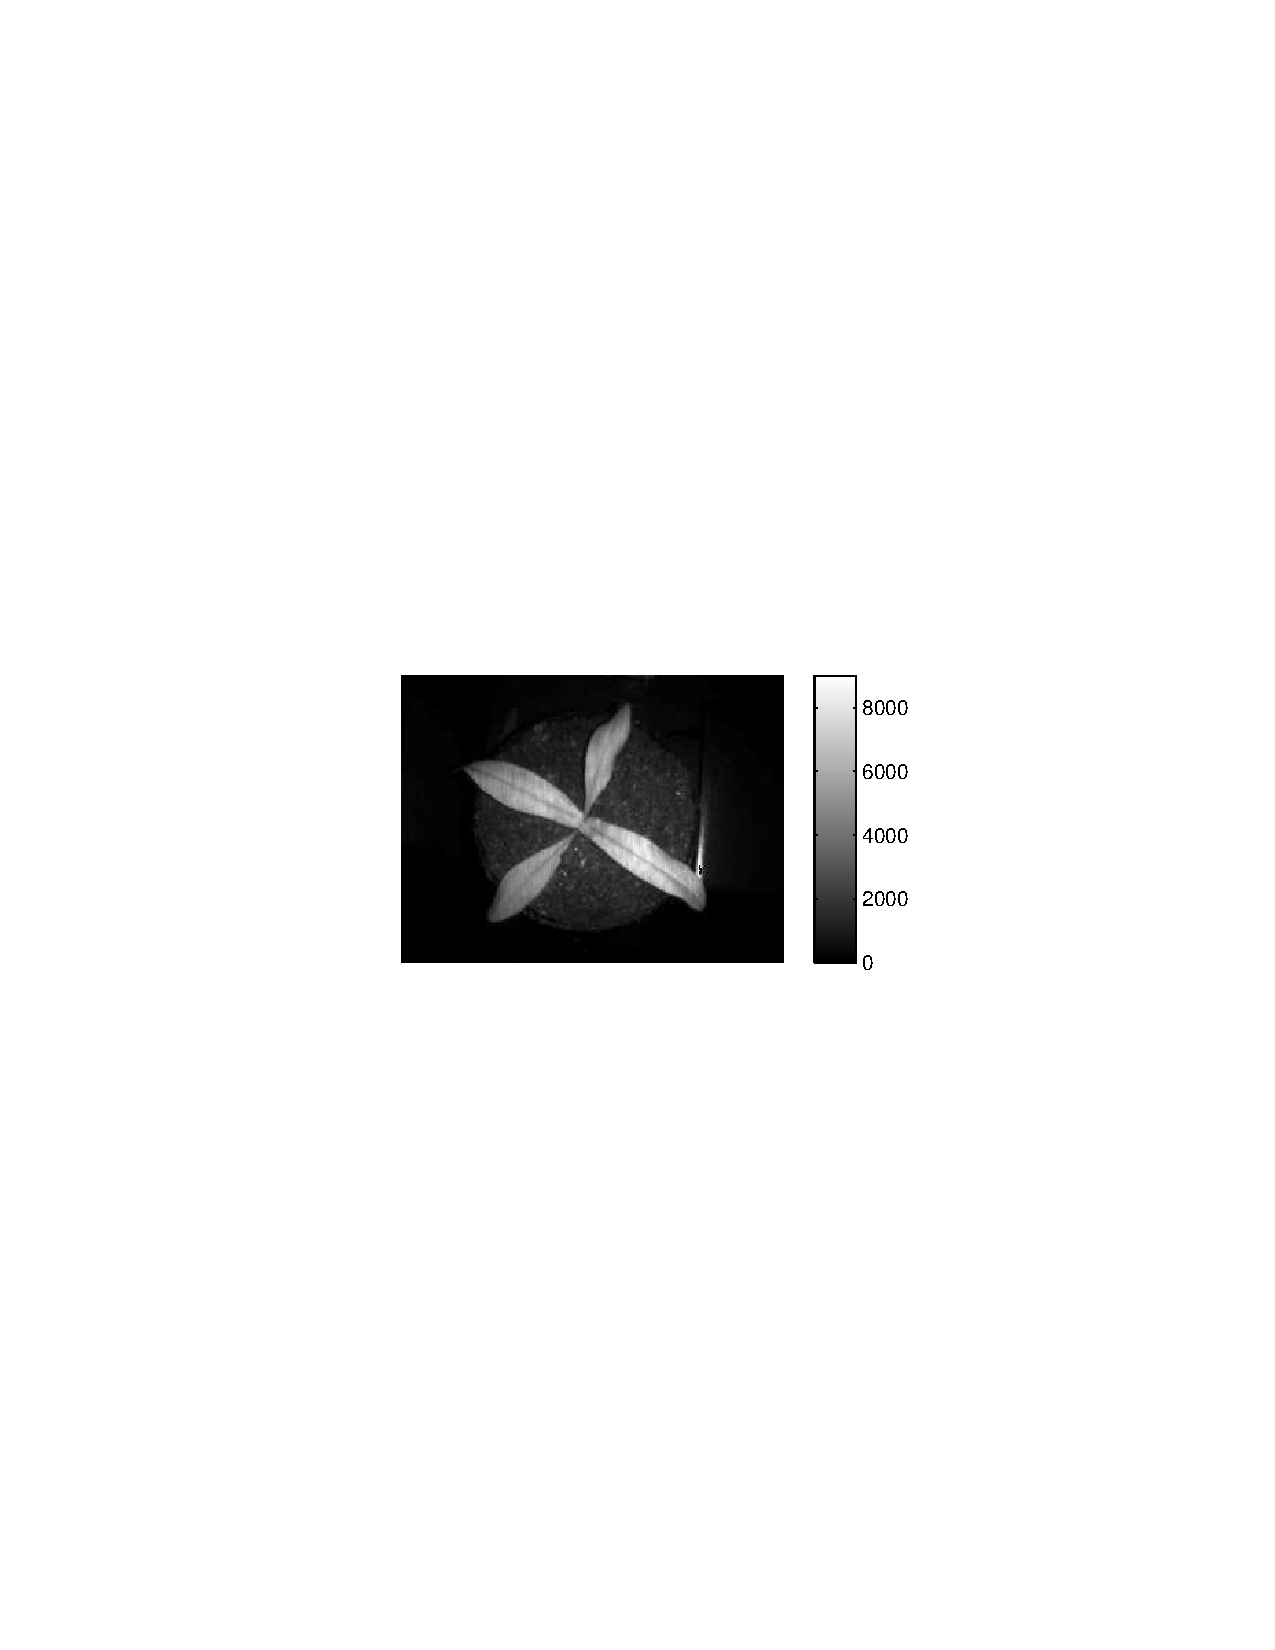
\includegraphics[trim=220 270 160 280,clip,width=0.4\linewidth]{Figures/plant1-ir} \\
($a$) & ($b$) \\
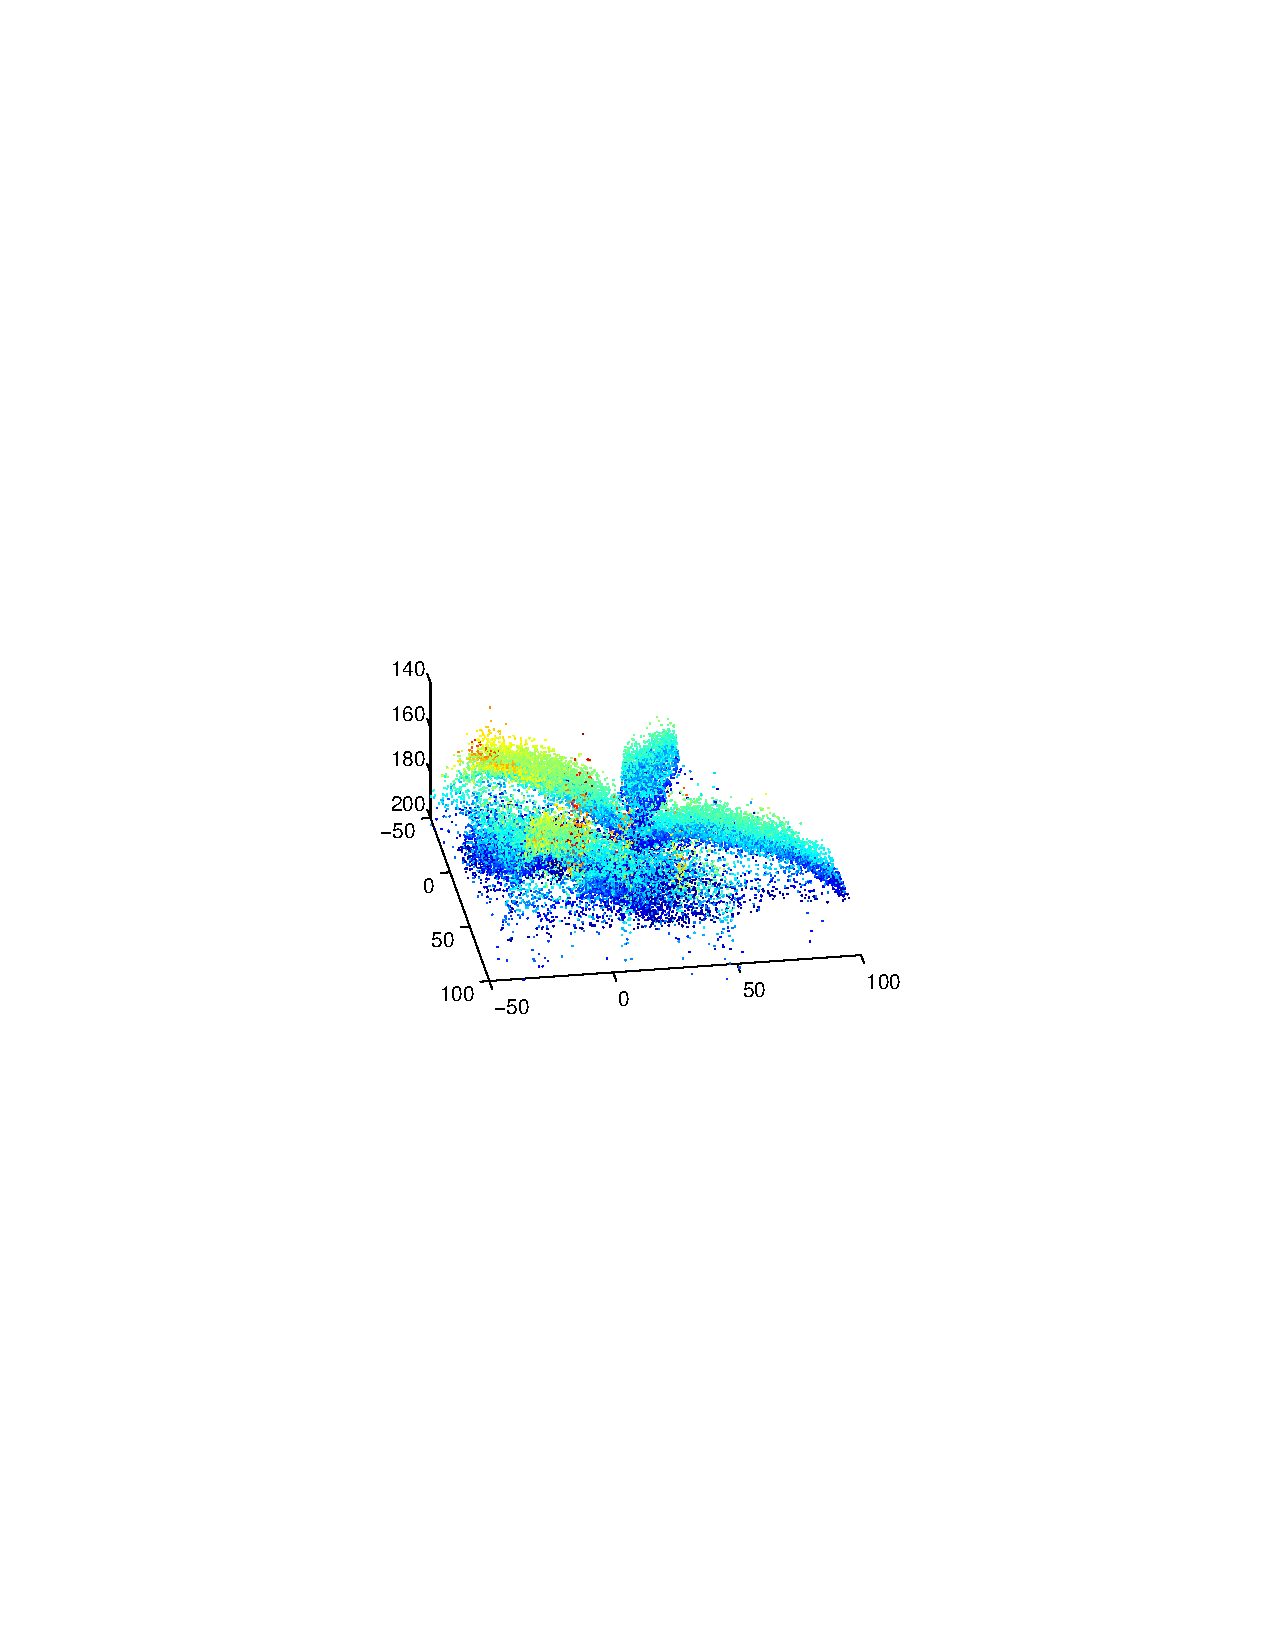
\includegraphics[trim=180 270 180 280,clip,width=0.4\linewidth]{Figures/plant1-3D-single} &
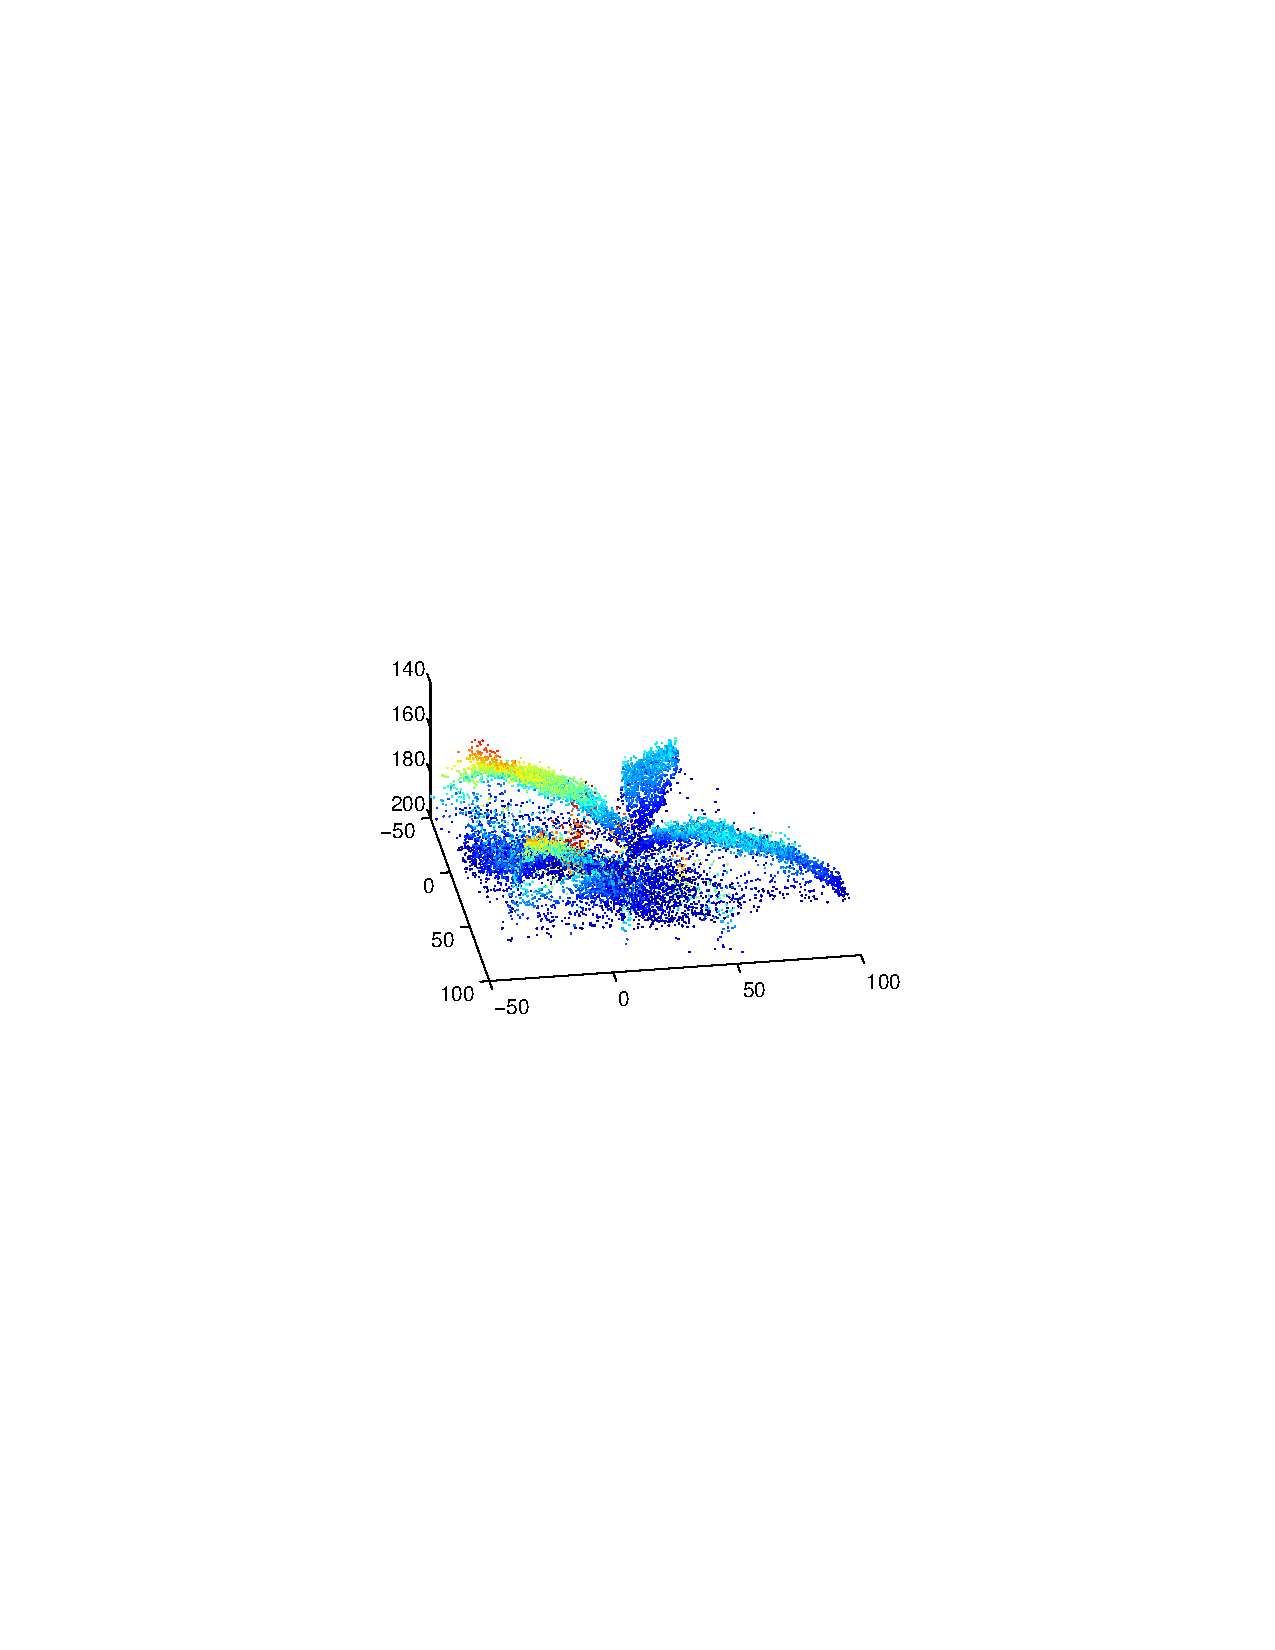
\includegraphics[trim=180 270 180 280,clip,width=0.4\linewidth]{Figures/plant1-3D-average} \\
($c$) & ($d$) \\
\end{tabular}
\end{center}
\caption{Illustration of sensor data.  ($a$) Portion of color image. ($b$) IR reflectance image with reflectance values. ($c$) Portion of a single depth image surrounding plant projected into $3$D showing significant depth noise. ($d$) Average of 60 depth images projected into $3$D, with $\sigma_S$ being the dominant source of noise.  Units of $3$D plots are mm.  The goal of this paper is to combine these data elements into }
\label{fig:plantnoise}
\end{figure}
